\section{Criterio 3: ENTROPIA}

Il criterio basato sull'entropia prevede di calcolare il contributo di ogni valore singolare mediante la seguente formula:
\begin{equation}
    f_j=\frac{\sigma_j^2}{\sum_{i=1}^{r}\sigma_i^2}
    \label{fj:contributi}
\end{equation}
e successivamente calcolare l'entropia totale della matrice mediante la seguente formula:
\begin{equation}
    E = -\frac{1}{\log(r)}\sum_{j=1}^r f_j \log(f_j)
\end{equation}

\noindent Con questo criterio, vengono selezionati i primi $\sigma_k$ valori singolari, dove $k$ viene scelto come il più piccolo indice tale che:
\begin{equation}
\sum_{j=1}^k f_i \geq E
\end{equation}

In questo caso l'entropia totale della matrice è risultata essere 0.517648. Volendo mantenere il 75\% dell'entropia totale il k suggerito è 116.
\begin{table}[H]
    \centering
    \begin{tabular}{|c|c|c|}
        \hline
        \textbf{Matrice} & \textbf{Righe} & \textbf{Colonne} \\
        \hline
        U\_troncata & 301 & 116 \\
        \hline
        S\_troncata & 116 & 116 \\
        \hline
        V\_troncata & 301 & 116 \\
        \hline
    \end{tabular}
    \caption{Dimensioni matrici troncate}
\end{table}

\begin{table}[H]
    \centering
    \begin{tabular}{|c|c|c|}
        \hline
        \textbf{Norma} &\textbf{Errore assoluto} \\
        \hline
        2 &  384.477333 \\
        \hline
        Frobenius & 2892.327572 \\
        \hline
    \end{tabular}
    \caption{Norme ed errori}
\end{table}

\noindent
E' noto inoltre che l'errore assoluto in norma due risulta essere $\sigma_{k+1}$ e in norma Frobenius 
\begin{equation}
    \sqrt{\sum_{i=k+1}^{r}\sigma_i^2}
\end{equation}
 dove k è il numero di valori singolari mantenuti.\\
Per la binarizzazione sono state utilizzate le seguenti soglie:
\begin{itemize}
    \item 0.25
    \item 0.5
    \item 0.75
    \item Soglia automatica calcolata con \textbf{graythresh}
\end{itemize}

\begin{figure}[H]
    \centering
     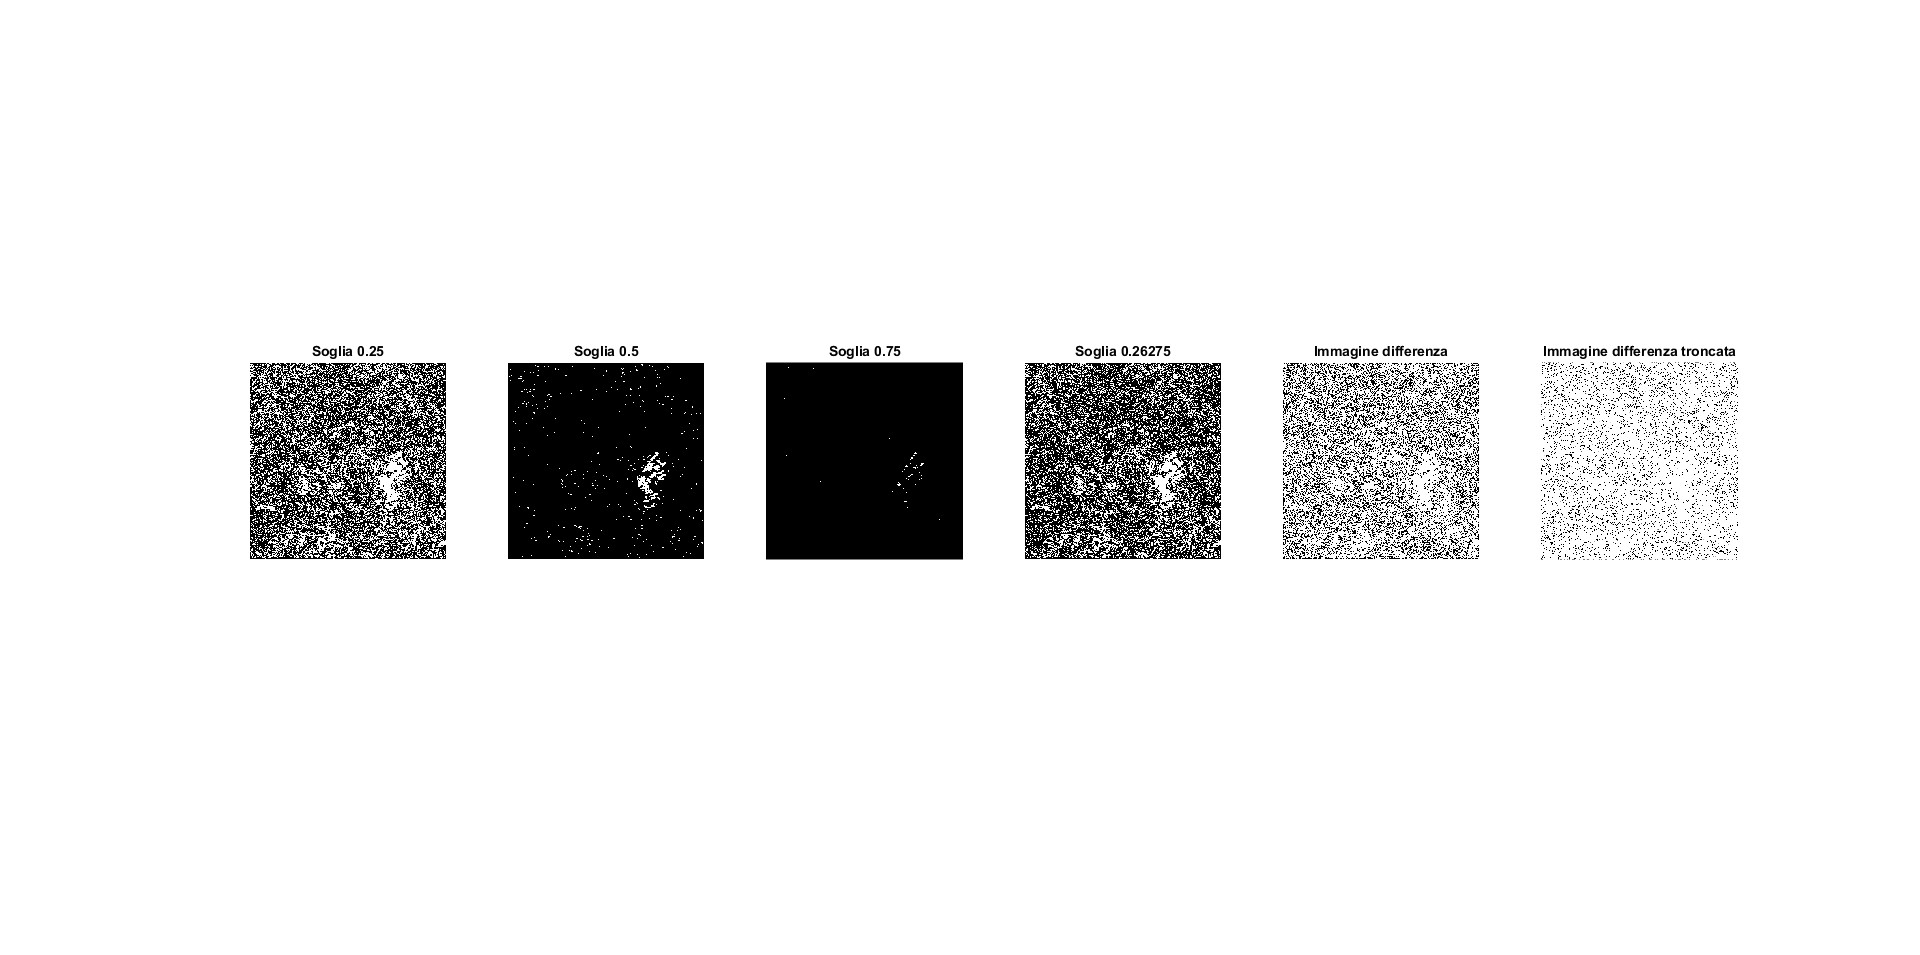
\includegraphics[width=\textwidth]{images/Criterio3.jpg}
    \caption{Immagini binarizzate con criterio 3}
\end{figure}

\noindent Le soglie 0.25 e automatica sono molto simili tra loro e sono "coerenti" sia con l'immagine originale che con quella troncata.

\noindent Per il processo di troncamento sono stati necessari in media circa \textcolor{blue}{\textbf{0.0009}} secondi.\\



